\documentclass{beamer}

\mode<presentation> {

  % The Beamer class comes with a number of default slide themes which
  % change the colors and layouts of slides. Below this is a list of
  % all the themes, uncomment each in turn to see what they look like.

%\usetheme{default}
%\usetheme{AnnArbor}
%\usetheme{Antibes}
%\usetheme{Bergen}
%\usetheme{Berkeley}
%\usetheme{Berlin}
%\usetheme{Boadilla}
%\usetheme{CambridgeUS}
%\usetheme{Copenhagen}
%\usetheme{Darmstadt}
%\usetheme{Dresden}
%\usetheme{Frankfurt}
%\usetheme{Goettingen}
%\usetheme{Hannover}
%\usetheme{Ilmenau}
%\usetheme{JuanLesPins}
%\usetheme{Luebeck}
\usetheme{Madrid}
%\usetheme{Malmoe}
%\usetheme{Marburg}
%\usetheme{Montpellier}
%\usetheme{PaloAlto}
%\usetheme{Pittsburgh}
%\usetheme{Rochester}
%\usetheme{Singapore}
%\usetheme{Szeged}
%\usetheme{Warsaw}

% As well as themes, the Beamer class has a number of color themes for
% any slide theme. Uncomment each of these in turn to see how it
% changes the colors of your current slide theme.

%\usecolortheme{albatross}
%\usecolortheme{beaver}
%\usecolortheme{beetle}
%\usecolortheme{crane}
%\usecolortheme{dolphin}
%\usecolortheme{dove}
%\usecolortheme{fly}
%\usecolortheme{lily}
%\usecolortheme{orchid}
%\usecolortheme{rose}
%\usecolortheme{seagull}
%\usecolortheme{seahorse}
%\usecolortheme{whale}
%\usecolortheme{wolverine}

%\setbeamertemplate{footline} % To remove the footer line in all slides uncomment this line
%\setbeamertemplate{footline}[page number] % To replace the footer line in all slides with a simple slide count uncomment this line

\setbeamertemplate{navigation symbols}{} % To remove the navigation symbols from the bottom of all slides uncomment this line
}

\usepackage{times}
\usepackage{graphicx}

\usepackage[utf8]{inputenc}
\usepackage[T1]{fontenc}
\usepackage{tikz}
\usepackage{algorithm}
\usepackage{algpseudocode}
\usepackage{pifont}

\usepackage{tree-dvips}
\usepackage{qtree}
\usepackage{tikz-qtree}
\usepackage{etoolbox}
\usepackage{pgfplots}
\usetikzlibrary{calc}

\newenvironment{figure*}%
{\begin{figure}}
{\end{figure}}


\title[RenderGirl]{\emph{RenderGirl} - A modular GPU raytracer using OpenCL for non-interactive graphics}

\author{Henrique Jung}
\institute[Unisinos]
{
Universidade do Vale do Rio dos Sinos \\
\medskip
\textit{henriquenj@gmail.com}
}
\date{\today}

\begin{document}

% remove "figures" prefix on figures
\setbeamertemplate{caption}{\raggedright\insertcaption\par}

\begin{frame}
\titlepage % Print the title page as the first slide
\end{frame}

\begin{frame}
\frametitle{Overview}
\tableofcontents
\end{frame}

\section{Introduction}

\begin{frame}
\frametitle{Introduction}

\begin{itemize}
\item Motivation

\begin{itemize}
\item Study the applications of GPU and GPU programming for non
  real-time graphics.
\item Offer more options for developers and users intersted in using
  dedicated hardware to perform their rendering.
\end{itemize}

\end{itemize}

\frametitle{Introduction}

\begin{itemize}
\item Objectives
\begin{itemize}
\item Create a raytracer capable of using specialized hardware while
  maintaining vendor agnosticism through OpenCL.
\item Design and implement a modular architecture with known
  interfaces capable of being plugged into a host 3D program.
\item Implement and study the applications of accelaration strucutres
  in the context of raytracing on many-core architectures, with focus
  on GPU.
\end{itemize}
\end{itemize}

\end{frame}


\section{Theory}
\begin{frame}
\frametitle{Theory}

\begin{itemize}

\item \emph{RenderGirl} is a raytracer renderer designed to run within the
OpenCL framework, which can take advantage of \emph{heteregenous
  platforms} consisting of GPUs, CPUs, FPGAs and some other types of
hardware.

\item Raytracing is a rendering algorithm based on the concept of
\emph{rays}, which are sent from a given point in space, creating the
concept of a camera. Each ray is tested against collision with the
objects in the scene, and if a collision is found, we may paint that
pixel with the color of the object.

\item Usually implemented with an accelaration structure that can
  apply a \emph{heuristic} in order optimize the rendering process.

\end{itemize}

\end{frame}



\section{Related work}
\begin{frame}
\frametitle{Related work}

Recent work related with GPU raytracing:

\begin{itemize}

\item Applications such as Blender Cycles, Octane render, V-ray
  renderer, Redshift and Indigo Renderer. Indigo and Cycles both claim
  to run using the OpenCL frmework.

\item Áfra and Szirmay-Kalos propose a novel traversal algorithm for
  BVH that doesn't use a stack\cite{Afra}.

\item Kalajanov and colleagues propose an acceleration structure using
  hierarchical two-level grids implemented in CUDA\cite{Kalojanov}.

\end{itemize}

\end{frame}


\begin{frame}
\frametitle{Related work}

\begin{itemize}

\item Ravichandran and colleagues propose a parallel divide and
  conquer raytracing suited for GPUs\cite{Ravichandran}.

\item Wong and colleagues propose an optimization method for GPU ray
  tracing by dividing objects into view-sets based on light and camera
  position\cite{Wong}.

\item Widmer and colleagues propose efficient hybrid acceleration
  structure for real-time screen space raytracing\cite{Widmer}.

\end{itemize}

\end{frame}

\section{RenderGirl}
\begin{frame}
\frametitle{RenderGirl}

\begin{itemize}

\item RenderGirl is composed of a \emph{core} that communicates with a
  given \emph{interface}.

\item The core portion is a static library that provides an API for
  receiving the 3D scene structure - vertices, triangles, objects,
  cameras and lights. It performs all of the communication between
  OpenCL and the interfaces, handling its context. It outputs an array
  of pixels with the rendered frame.

\item Interfaces link with the core at compile time and provide
  communication with a given host program.

\end{itemize}

\end{frame}

\begin{frame}
  \frametitle{RenderGirl}

Features supported:

\begin{itemize}
\item Rendering of triangulated scenes composed of several objects
\item Flat shading
\item OBJ-like materials (except on Blender plugin)
\item FXAA implemented in OpenCL
\item BVH partioning structure that optimizes the rendering process.
\end{itemize}

\end{frame}

\subsection{RenderGirl architecture}
\begin{frame}
\frametitle{RenderGirl architecture}

\begin{figure}
\centering
\usetikzlibrary{positioning,calc,fit}

\definecolor{black_red}{RGB}{179,0,0}
\definecolor{black}{RGB}{0,0,0}
\definecolor{blue}{RGB}{0,51,153}
\definecolor{orange}{RGB}{255,128,0}


\pgfdeclarelayer{core}
\pgfdeclarelayer{runtime}
\pgfsetlayers{core,main}

\pgfkeys{
  /tikz/node distance/.append code={
    \pgfkeyssetvalue{/tikz/node distance value}{#1}
  }
}

\newlength\myframesep
\setlength\myframesep{0pt}

\newcommand\widernode[5][core_node]{
\node[
        #1,
        inner sep=0pt,
        shift=($(#2.south)-(#2.north)$),
        yshift=-\pgfkeysvalueof{/tikz/node distance value},
        fit={(#2) (#3)},
        label=center:{\color{white}#4}] (#5) {};
}
% fix widernodeabove function, right now will shift nodes on X axis
\newcommand\widernodeabove[5][core_node]{
\node[
        #1,
        inner sep=0pt,
        shift=($(#2.north)+(#2.north)$),
        yshift=+\pgfkeysvalueof{/tikz/node distance value},
        fit={(#2) (#3)},
        label=center:{\color{white}#4}] (#5) {};
}

\begin{tikzpicture}[node distance=3pt,outer sep=0pt,
core_node/.style={
  draw=black,
  fill=black_red,
  rounded corners,
  font={\color{white}},
  align=center,
  minimum width = 70pt,
  text height=12pt,
  text depth=6pt},
other_node/.style={
  fill=black,
  draw=black,
  rounded corners,
  font={\color{white}},
  align=center,
  minimum width = 60pt,
  text height=12pt,
  text depth=6pt},
interface_node/.style={
  fill=orange,
  draw=black,
  rounded corners,
  font={\color{white}},
  align=center,
  minimum width = 70pt,
  text height=12pt,
  text depth=6pt},
host_node/.style={
  fill=black,
  draw=black,
  rounded corners,
  font={\color{white}},
  align=center,
  minimum width = 216pt,
  text height=12pt,
  text depth=6pt},
]

% core nodes

\node[core_node] (log) {Log subsystem};
\node[core_node, right=of log] (scene) {Scene Manager};
\node[core_node, right=of scene] (shared) {RenderGirl shared};
\widernode{log}{scene}{OpenCl wrapper}{wrapper};
\node[core_node, below=of shared] (kernels) {Kernels};

% interface

\node[interface_node, above=of scene](wrapper_host){Host structures};
\node[interface_node, above=of log](listeners){Log Listeners};
\node[interface_node, above=of shared](flow){Flow control};

\begin{pgfonlayer}{core}
\draw[core_node,draw=black,fill=black_red!40]
 ([xshift=-\myframesep,yshift=3\myframesep]current bounding box.north west)
    rectangle
  ([xshift=\myframesep,yshift=-\myframesep]current bounding box.south east);
\end{pgfonlayer}

% opencl runtime nodes

\widernode[other_node]{wrapper}{wrapper}{OpenCL runtime driver}{runtime}
\node[other_node, below=of kernels](compiler){OpenCL Compiler};

%  hardware

\widernode[other_node]{runtime}{compiler}{Hardware}{hardware}

% host 3d software

\node[host_node, above=of wrapper_host](host){Host 3D software};

\end{tikzpicture}
\caption{Architecture of RenderGirl. Red represents core components,
  orange represents interface components.}
\label{fig:architecture}
\end{figure}

\end{frame}


\begin{frame}
\frametitle{RenderGirl architecture}
\begin{itemize}
\item It was developed three interfaces: console interface, wxWidgets
  interface and a Blender Plugin interface.
\item The focus was to make an unmodified core works on all these
  interfaces.
\item Challanges with Blender since it only provides a Python API.
\end{itemize}
\end{frame}


\subsection{Bounding volume hierarchy}
\begin{frame}
  \frametitle{Bounding volume hierarchy}
\begin{itemize}
\item It was used BVHs as acceleration structures, which was chosen
  based on a study conducted by Thrane and Simonsen comparing three
  different acceleration structures on GPUs: bounding volume
  hierarchies, kd-trees and uniform grids. In their results BVH
  outperforms the other
  two\cite{Thrane}. %TODO: every time I cite this guy is a new errro, why?
\item Divided into two main portions: \emph{construction} and \emph{traversal}.
\item Construction is done at CPU once per frame and it's
  serialized. Based on the algorithm developed by original authors of
  BVH: Kay and Kajiya\cite{kay1986ray}.
\item Traversal is done at GPU using an algorithm developed by Thrane
  and Simonsen.
\end{itemize}

\end{frame}


\subsubsection{BVH construction}
\begin{frame}
  \frametitle{BVH construction}
\begin{figure*}
\centering
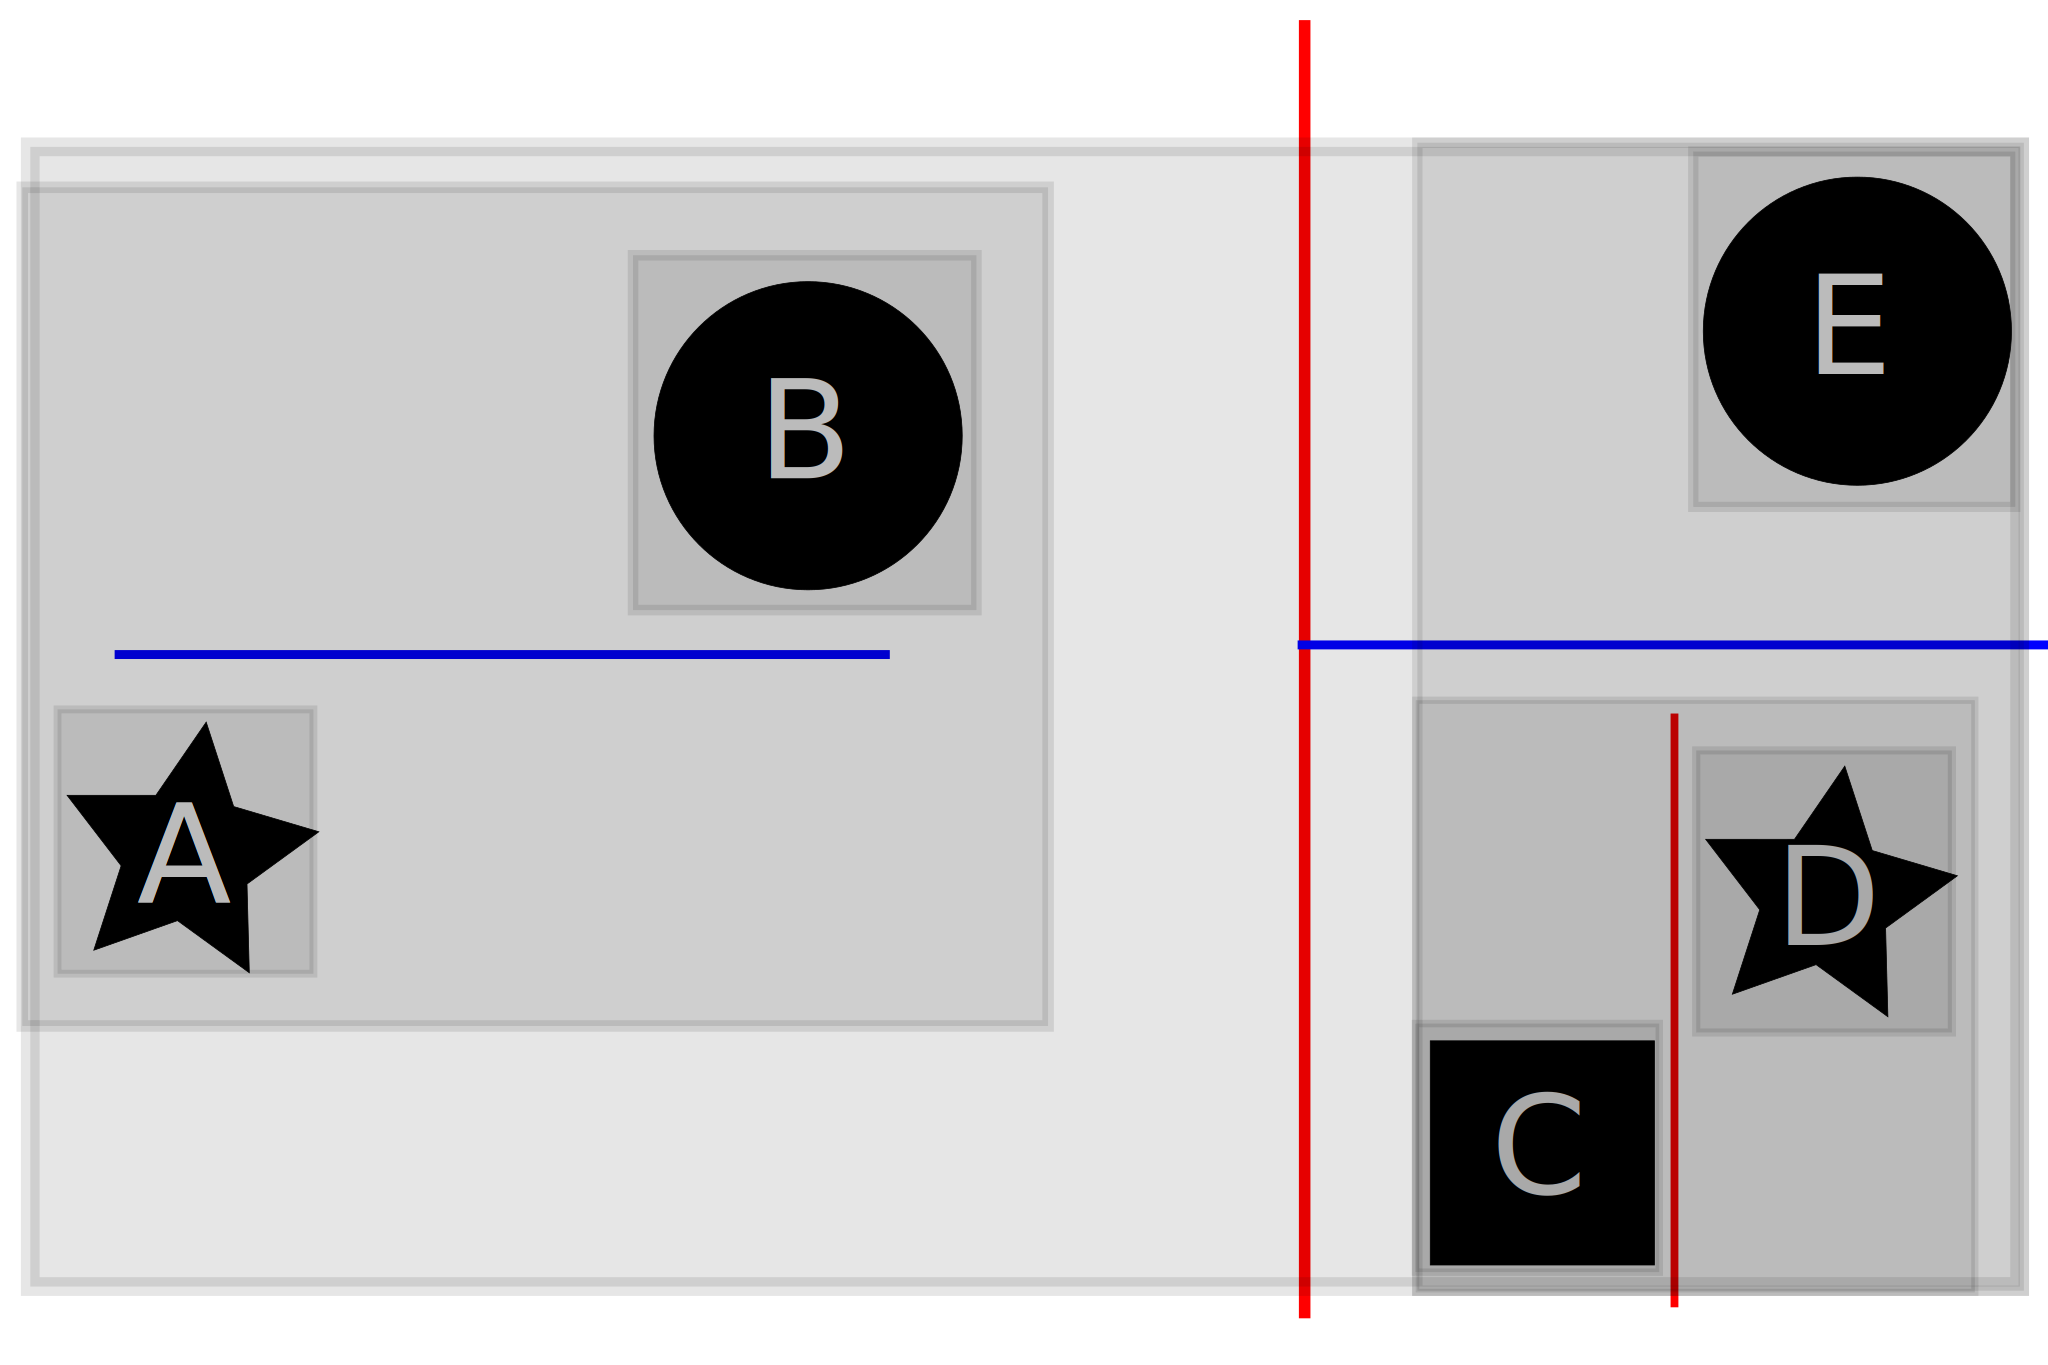
\includegraphics[width=0.8\textwidth]{bvh-construction.png}
\caption{The BVH visualized on a scene, with each level's AABB. Red
  bars represent an X split and blue bars Y splits}
\label{fig:bvh-construction}
\end{figure*}

\end{frame}


\subsubsection{BVH traversal}
\begin{frame}
  \frametitle{BVH traversal}
\begin{figure}
\centering
\newrobustcmd*{\square}[1]{\tikz{\filldraw[draw=#1,fill=#1] (0,0)
rectangle (0.2cm,0.2cm);}}

\newrobustcmd*{\mycircle}[1]{\tikz{\filldraw[draw=#1,fill=#1] (0,0) circle [radius=0.1cm];}}

\newrobustcmd*{\mytriangle}[1]{\tikz{\filldraw[draw=#1,fill=#1] (0,0) --
(0.2cm,0) -- (0.1cm,0.2cm);}}

\begin{tikzpicture}[sibling distance=20pt]
\tikzset{level distance=30pt}
\Tree[.\node(0){0}; [.\node(1){1}; [.\node(2){2}; \mytriangle{red}A ]
               [.\node(3){3}; \mytriangle{red}B ]]
          [.\node(4){4}; [.\node(5){5}; \mytriangle{red}C ]
                [.\node(6){6};
                [.\node(7){7}; [.\node(8){8}; \mytriangle{red}D ][.\node(9){9}; \mytriangle{red}E ]]
                [.\node(10){10}; [.\node(11){11}; \mytriangle{red}F ]
                [.\node(12){12}; \mytriangle{red}G ]]]]]
\node [anchor=base, right=14em]  (13) {13};
\draw[semithick,dashed,->] (1.east) to (4.west);
\draw[semithick,dashed,->] (2.east) to (3.west);
\draw[semithick,dashed,->] (3.east) to (4.west);
\draw[semithick,dashed,->] (5.east) to (6.west);
\draw[semithick,dashed,->] (7.east) to (10.west);
\draw[semithick,dashed,->] (8.east) to (9.west);
\draw[semithick,dashed,->] (7.east) to (10.west);
\draw[semithick,dashed,->] (9.east) to (10.west);
\draw[semithick,dashed,->] (11.east) to (12.west);
\draw[semithick,dashed,->] (0.east) to (13.west);
\draw[semithick,dashed,->] (4.east) to (13.west);
\draw[semithick,dashed,->] (6.east) to (13.south);
\draw[semithick,dashed,->] (10.north) to (13.south);
\draw[semithick,dashed,->] (12.north) to (13.south);

\end{tikzpicture}


\caption{Visualization of the BVH}
\label{fig:bvh}
\end{figure}

\end{frame}



\section{Results}
\begin{frame}
  \frametitle{Results}

Several scenes were tested with increasing resolutions:
\begin{itemize}
\item Scene 1: A scene depicting several tables and some kitchen
  objects evenly distributed. It contains 203.644 vertices, 405.242
  triangles divided into 233 objects.
\item Scene 2: A scene with a single whale object containing 8.432
  vertices and 16.764 triangles.
\item Scene 3: A scene depicting a cabin. It contains 93.570 vertices,
  178.104 triangles divided into 250 objects.
\end{itemize}
\end{frame}

\begin{frame}
  \frametitle{Results}

\begin{figure}
\centering
\begin{tikzpicture}
\begin{axis}[
    title={The time of rendering for each scene},
    xlabel={Resolution},
    ylabel={Milliseconds},
    xmin=0, xmax=2500,
    ymin=0, ymax=4000,
    xtick={0, 500,1000,1500,2000},
    ytick={0,1000,2000,3000,4000},
    legend pos=north west,
    ymajorgrids=true,
    grid style=dashed,
    scaled ticks=false, tick label style={/pgf/number format/fixed},
    legend entries={Kitchens,Whale,Cabin},
]
% scene 1
\addplot[color=red,mark=*,mark size = 1,dashed,nodes near coords]
    coordinates {(500,296)(1000, 375)(1500,501)(2000,695)};
%scene 2
\addplot[color=blue,mark=*,mark size = 1,dashed,nodes near coords, nodes near coords align={horizontal}]
    coordinates {(500,203)(1000, 829)(1500,1875)(2000,3227)};
% scene 3
\addplot[color=violet,mark=*,mark size = 1,dashed,nodes near coords=\raisebox{0.1cm}{\pgfmathprintnumber\pgfplotspointmeta}]
    coordinates {(500,314)(1000,779)(1500,1521)(2000,2540)};

\end{axis}
\end{tikzpicture}
\caption{Rendering time of the three scenes across different
  resolutions. Resolution value represents both width and height.}
\label{fig:scenes-results}
\end{figure}


\end{frame}


\begin{frame}
  \frametitle{Results}
\begin{figure*}
\centering
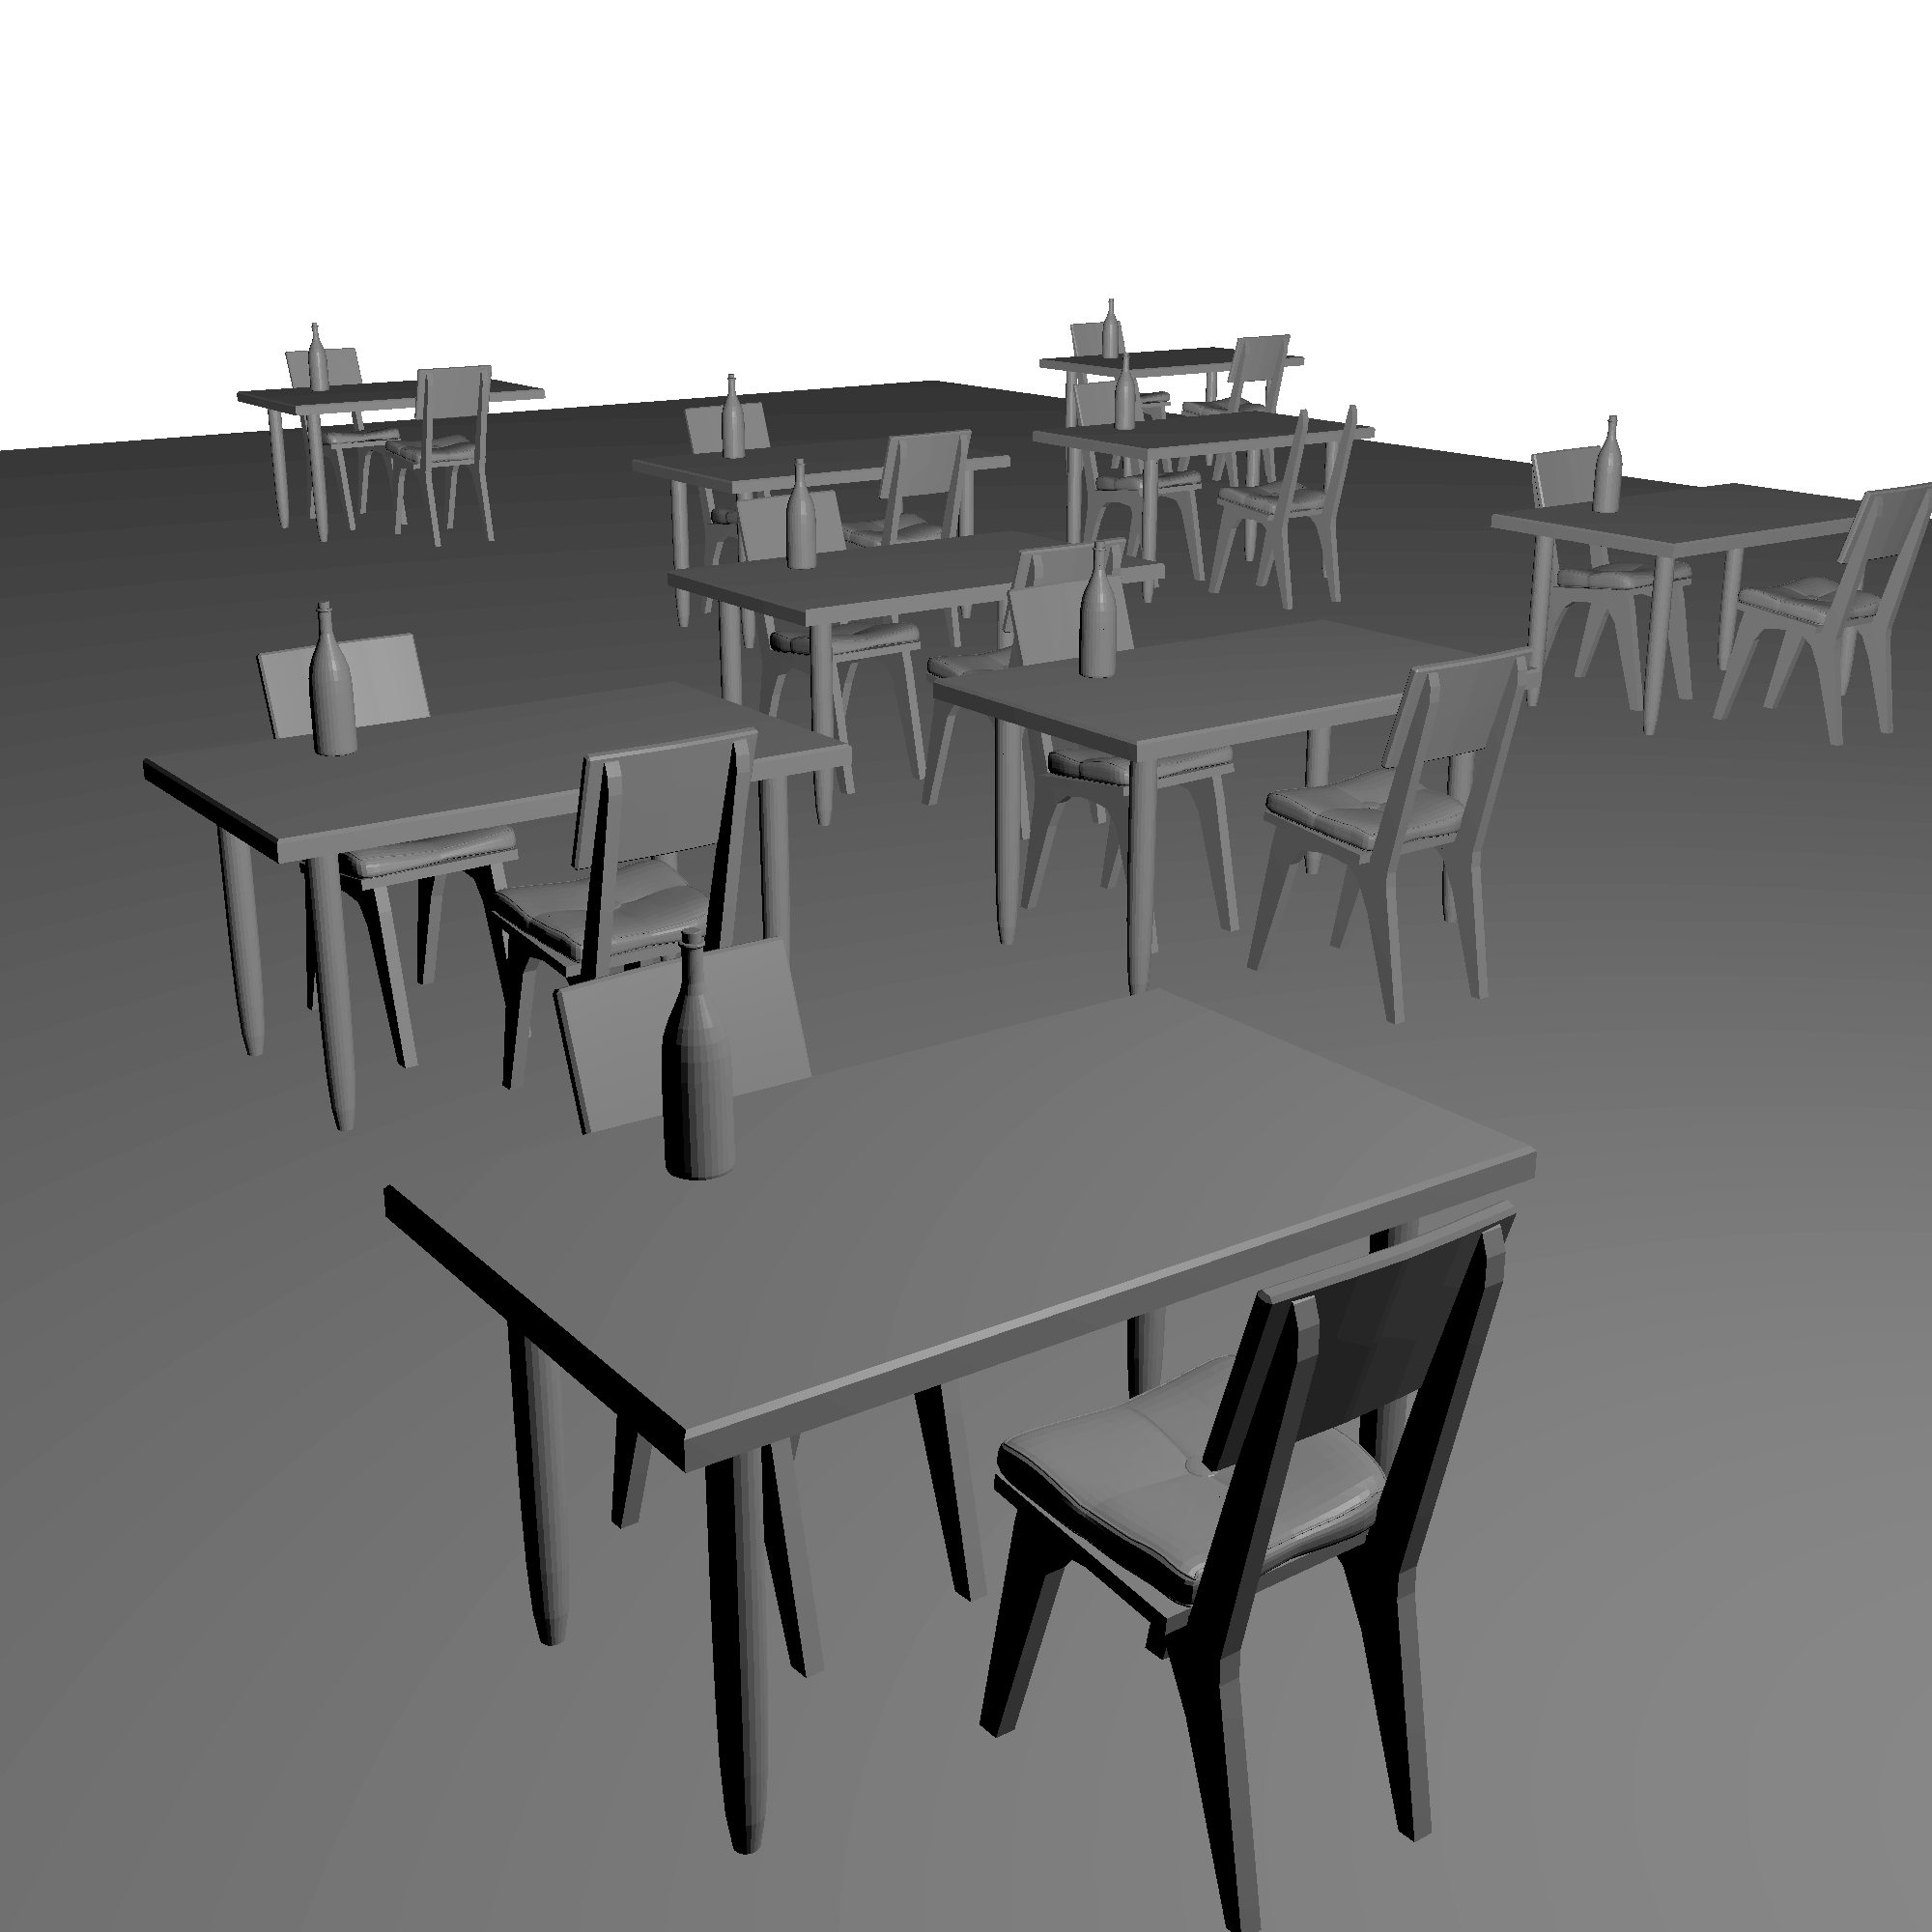
\includegraphics[width=0.6\textwidth]{several_kitchen.png}
\caption{Kitchens: 203.644 vertices, 405.242 triangles divided into
  233 objects.}
\end{figure*}
\end{frame}



\begin{frame}
  \frametitle{Results}
\begin{figure*}
\centering
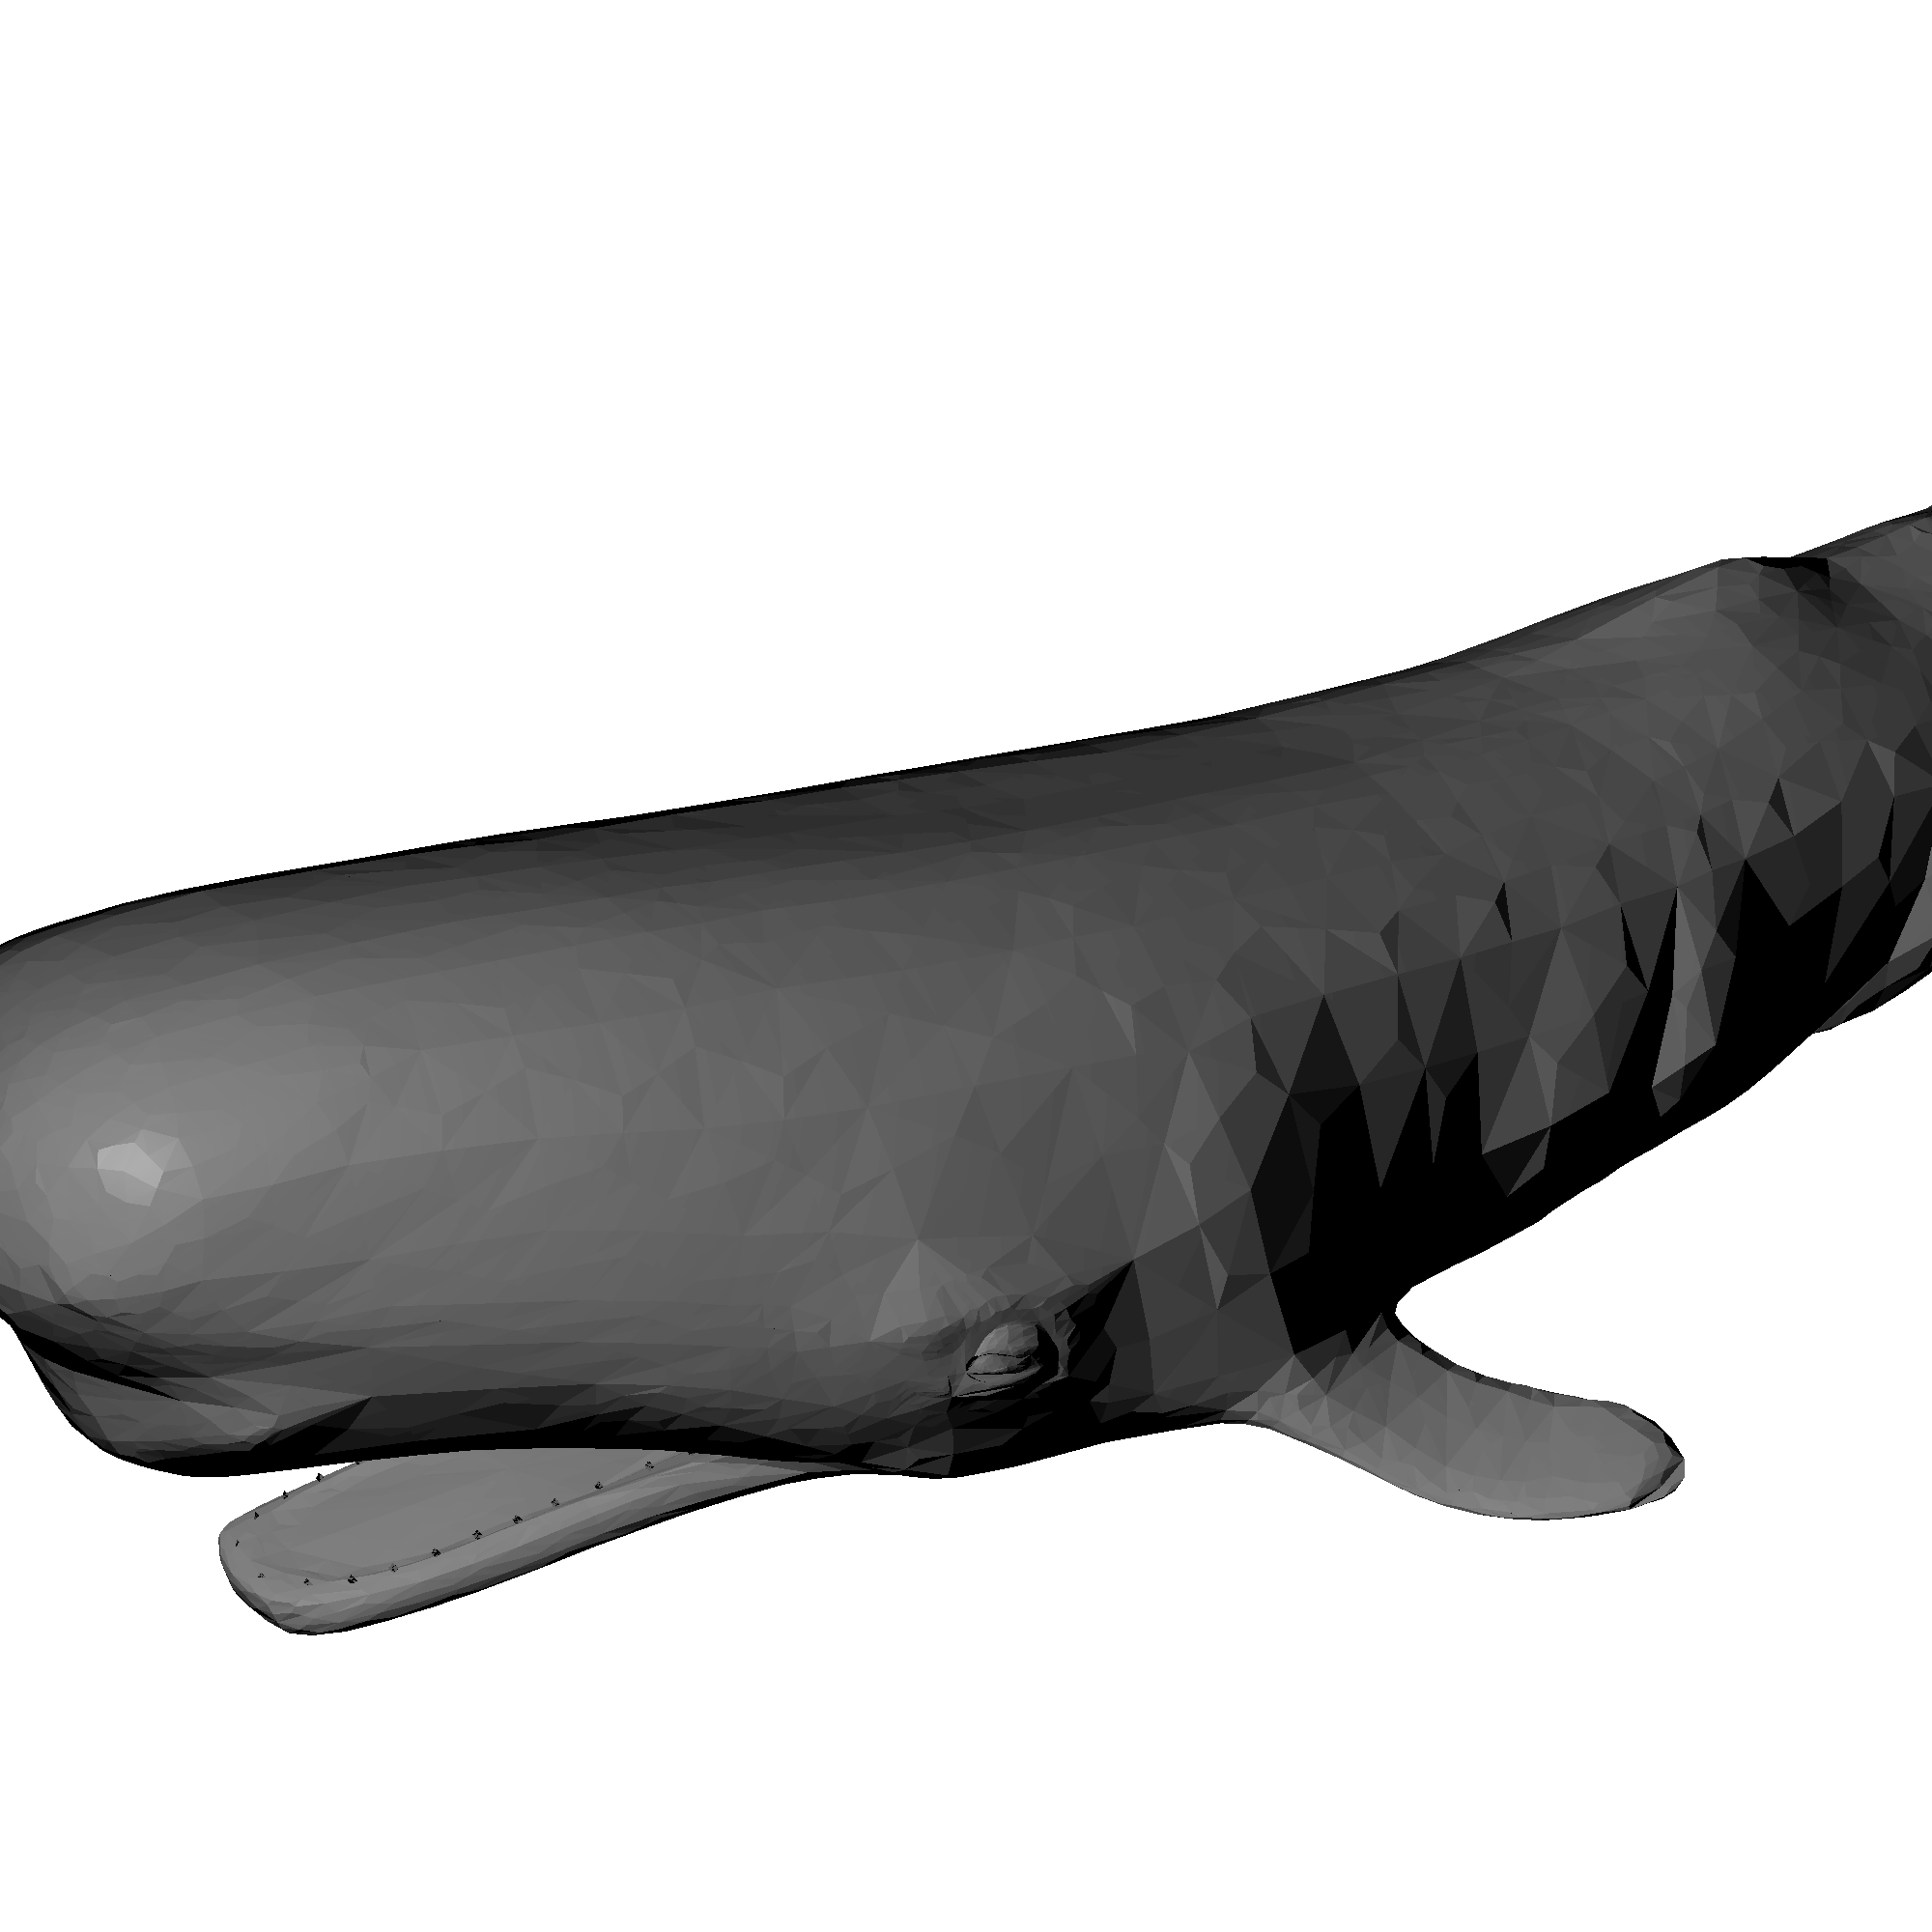
\includegraphics[width=0.6\textwidth]{whale.png}
\caption{Whale: single object, 8.432 vertices and 16.764 triangles.}
\end{figure*}
\end{frame}


\begin{frame}
  \frametitle{Results}
\begin{figure*}
\centering
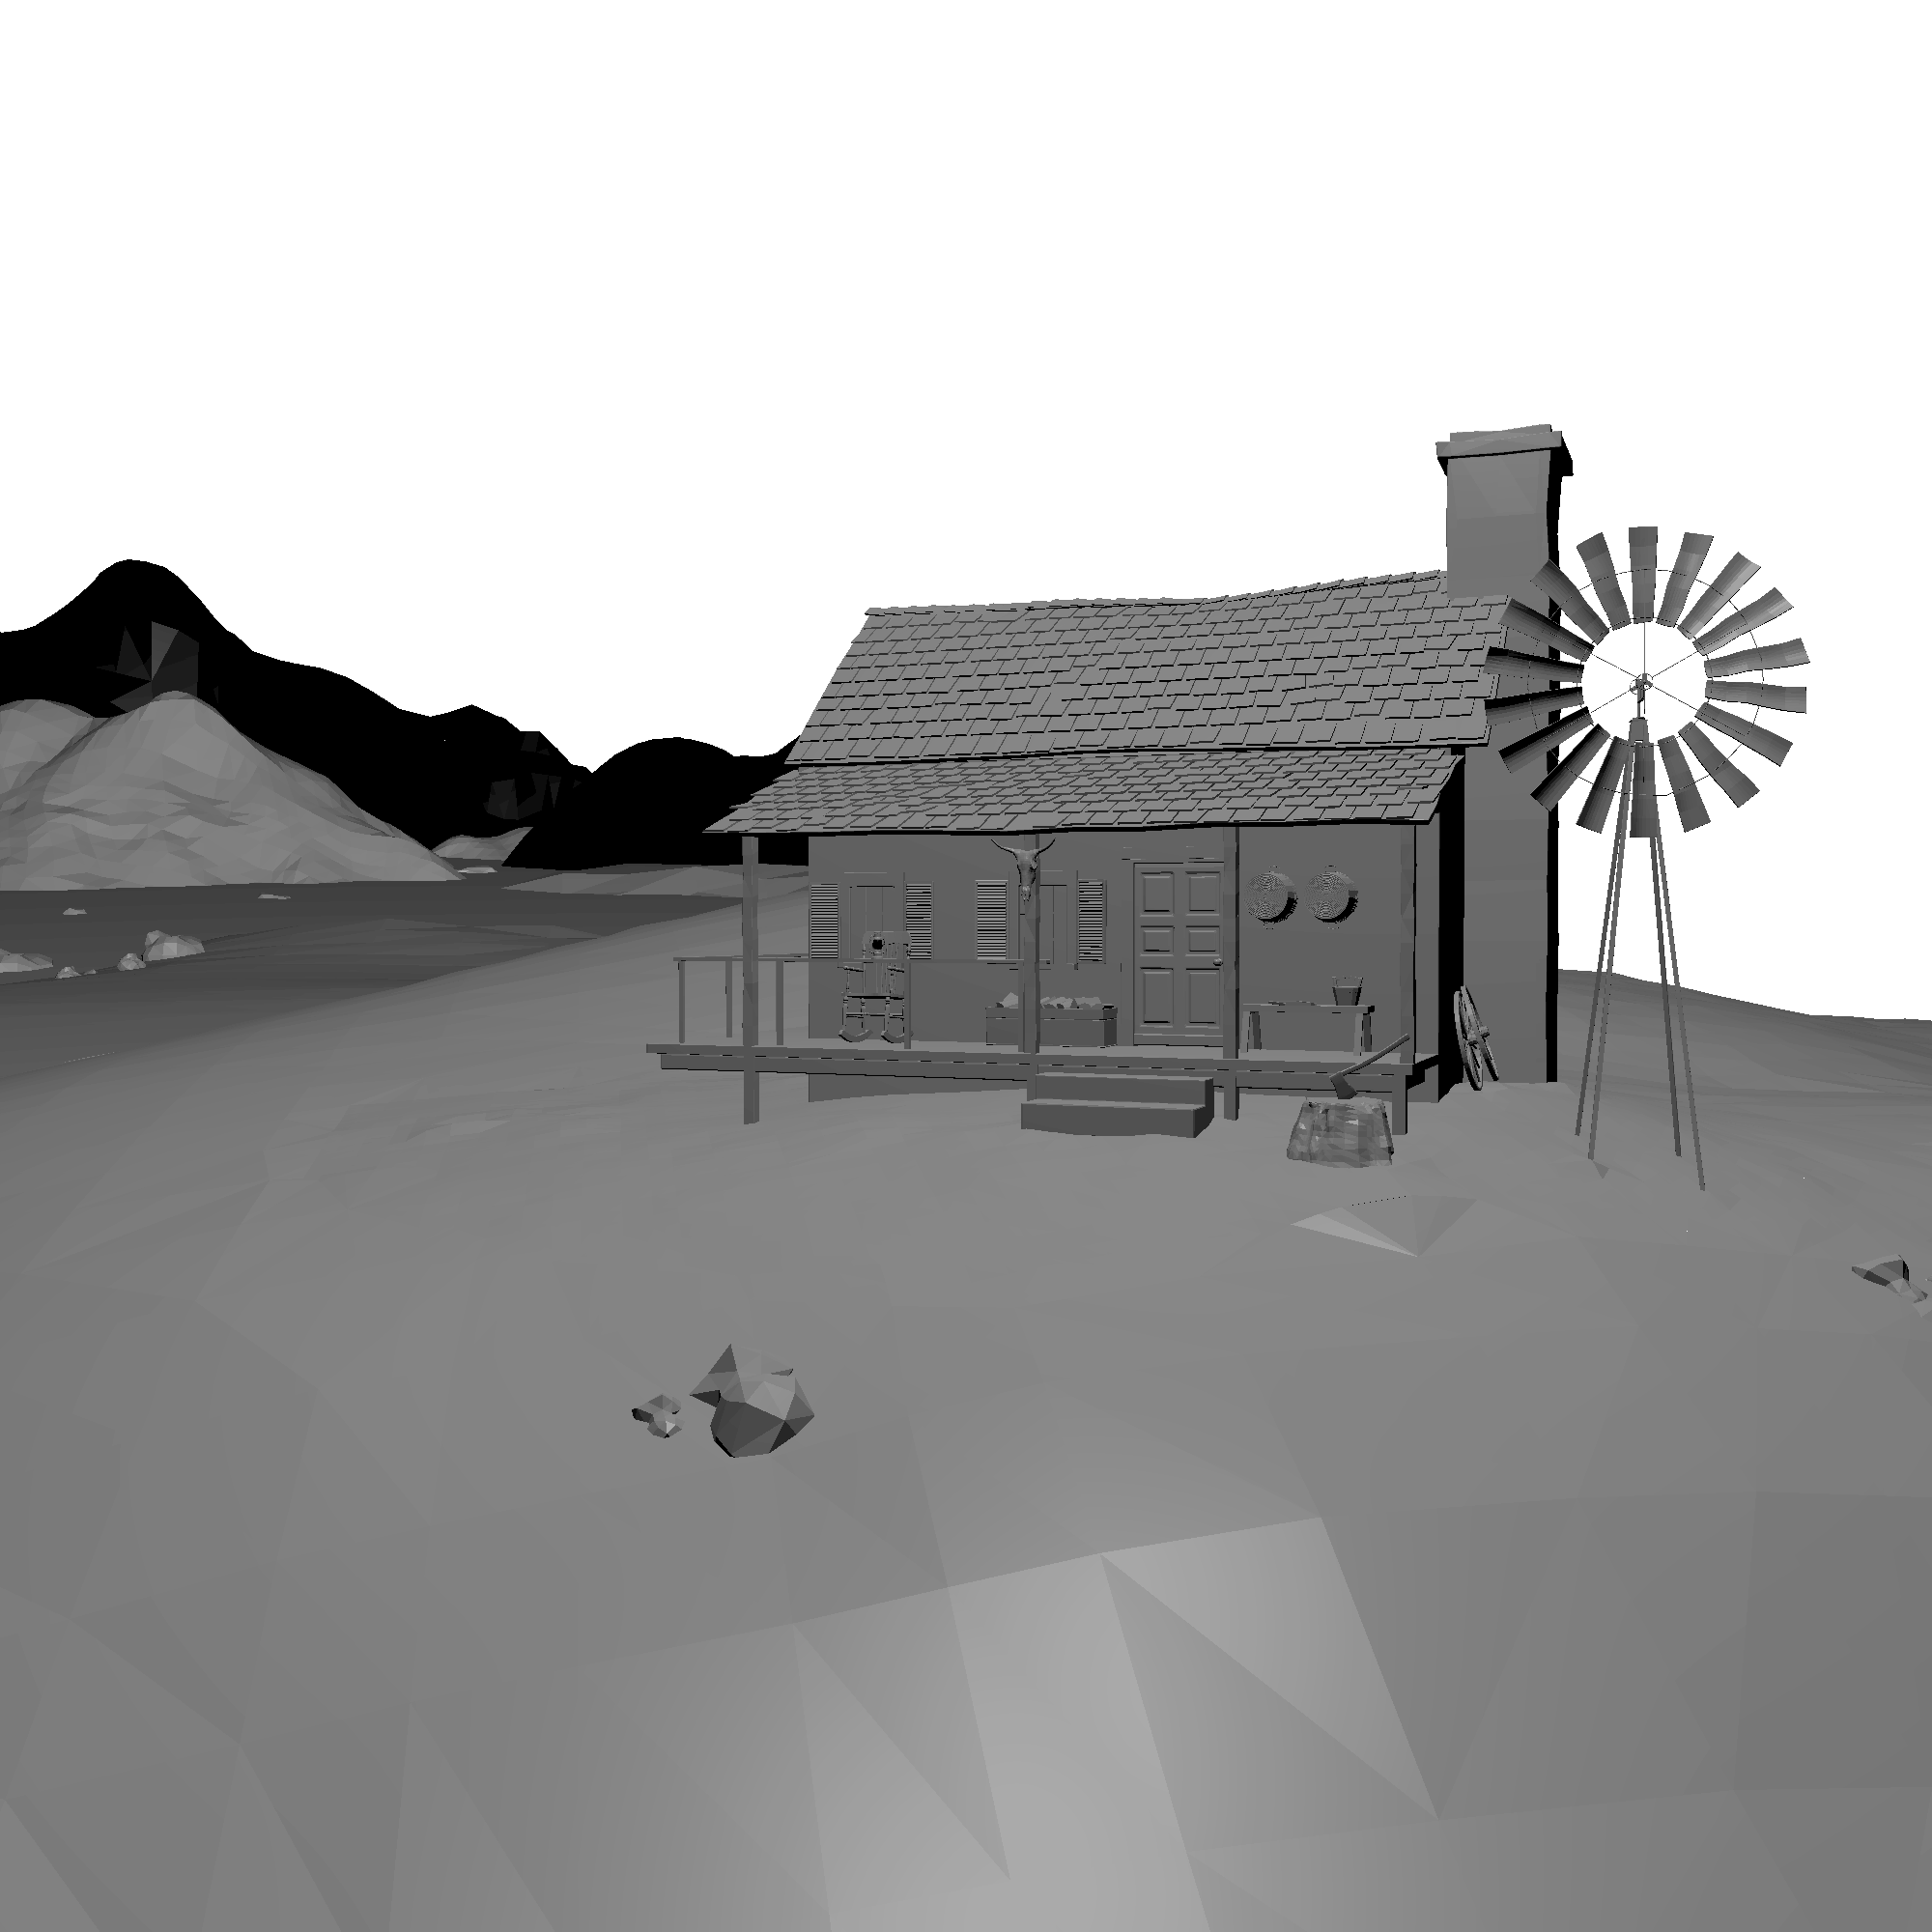
\includegraphics[width=0.6\textwidth]{cabin.png}
\caption{Cabin: 93.570 vertices, 178.104 triangles divided into 250
  objects}
\end{figure*}
\end{frame}


\section{Future work}
\begin{frame}
  \frametitle{Future work}

\begin{itemize}
\item Distribute render into \emph{passes}.
\item Optimize the Python side of the Blender plugin.
\item Implement an hybrid structure that would also split objects that it considers too big for the scene.
\begin{itemize}
\item This would need to take into consideration the overall flow of
  the raytracer.
\end{itemize}
\end{itemize}

\end{frame}


% TODO add memory layout
% TODO add traversal algorithm

\begin{frame}[allowframebreaks]
\frametitle{References}
\bibliographystyle{amsalpha}    %TODO: fix references markers on
                                %slides
\bibliography{references}
\end{frame}

\end{document}
